\documentclass[11pt]{article} \usepackage{fullpage} \usepackage{graphicx} \usepackage{epstopdf} \usepackage{color} \usepackage{psfrag} \usepackage{pdfsync}\usepackage{indentfirst}\usepackage{subfigure}\usepackage{float}\usepackage[section]{placeins}
\usepackage{enumerate}
\usepackage{multirow}
\usepackage{amsfonts, fullpage, graphics} 
\usepackage{algorithm,algorithmic}
\usepackage{amsmath,amssymb,amsthm,bm,hyperref}
\usepackage{dsfont}
\usepackage[parfill]{parskip}
\usepackage[margin=1in]{geometry}
\newcommand{\Lagr}{\mathcal{L}}
\newcommand{\norm}[1]{\left\lVert#1\right\rVert}
\newcommand{\floor}[1]{\lfloor #1 \rfloor}
\newcommand{\todo}[1]{}
\renewcommand{\todo}[1]{{\color{red} TODO: {#1}}}
\newcommand\independent{\protect\mathpalette{\protect\independenT}{\perp}}
\newcommand{\obar}[1]{\mkern 1.5mu\overline{\mkern-1.5mu#1\mkern-1.5mu}\mkern 1.5mu}
\def\independenT#1#2{\mathrel{\rlap{$#1#2$}\mkern2mu{#1#2}}}
\newcommand{\rpm}{\sbox0{$1$}\sbox2{$\scriptstyle\pm$}
  \raise\dimexpr(\ht0-\ht2)/2\relax\box2 }
\usepackage{xspace}
\newcommand{\latex}{\LaTeX\xspace}
\setlength{\parindent}{2em}

\usepackage{listings}
\usepackage{color} %red, green, blue, yellow, cyan, magenta, black, white
\definecolor{mygreen}{RGB}{28,172,0} % color values Red, Green, Blue
\definecolor{mylilas}{RGB}{170,55,241}
\DeclareMathOperator{\E}{\mathbb{E}}
\DeclareMathOperator*{\argmax}{arg\,max}
\DeclareMathOperator*{\argmin}{arg\,min}

\begin{document}

{\parindent 0pt \begin{tabular}[t]{l} 16-720 Computer Vision \\ Spring 2020 \end{tabular}}%  \hfill XX/XX/14 \vskip 0.2in }
\parindent 0pt \parskip 8pt
\begin{center} \large\bf Homework 1 \end{center}
\begin{center} \large\bf Zongwen Mu, Andrew ID: zongwenm \end{center}
\bigskip


\section{Representing the World with Visual Words}

\setcounter{subsection}{0}
\subsection{Extracting Filter Responses}

\setcounter{subsubsection}{0}
\subsubsection{}

\setlength{\parindent}{2em} The Gaussian filter reduces the noises and high frequency responses in images, which would make it easier for classifier to find similarities between images.

The derivative of Gaussian filter in X direction picks up distinct vertical features.

The derivative of Gaussian filter in Y direction picks up distinct horizontal features.

The Gaussian Laplacian filter picks up the contours in the images.

We need multiple scales of filter response so that the classifier could work with images with different sizes.

\setcounter{subsubsection}{1}
\subsubsection{}

Set default scales as $\left[ \begin{smallmatrix} 1 & 2 & 4 \end{smallmatrix} \right]$, the collage of images is shown below:

\begin{figure}[htb]
\centering
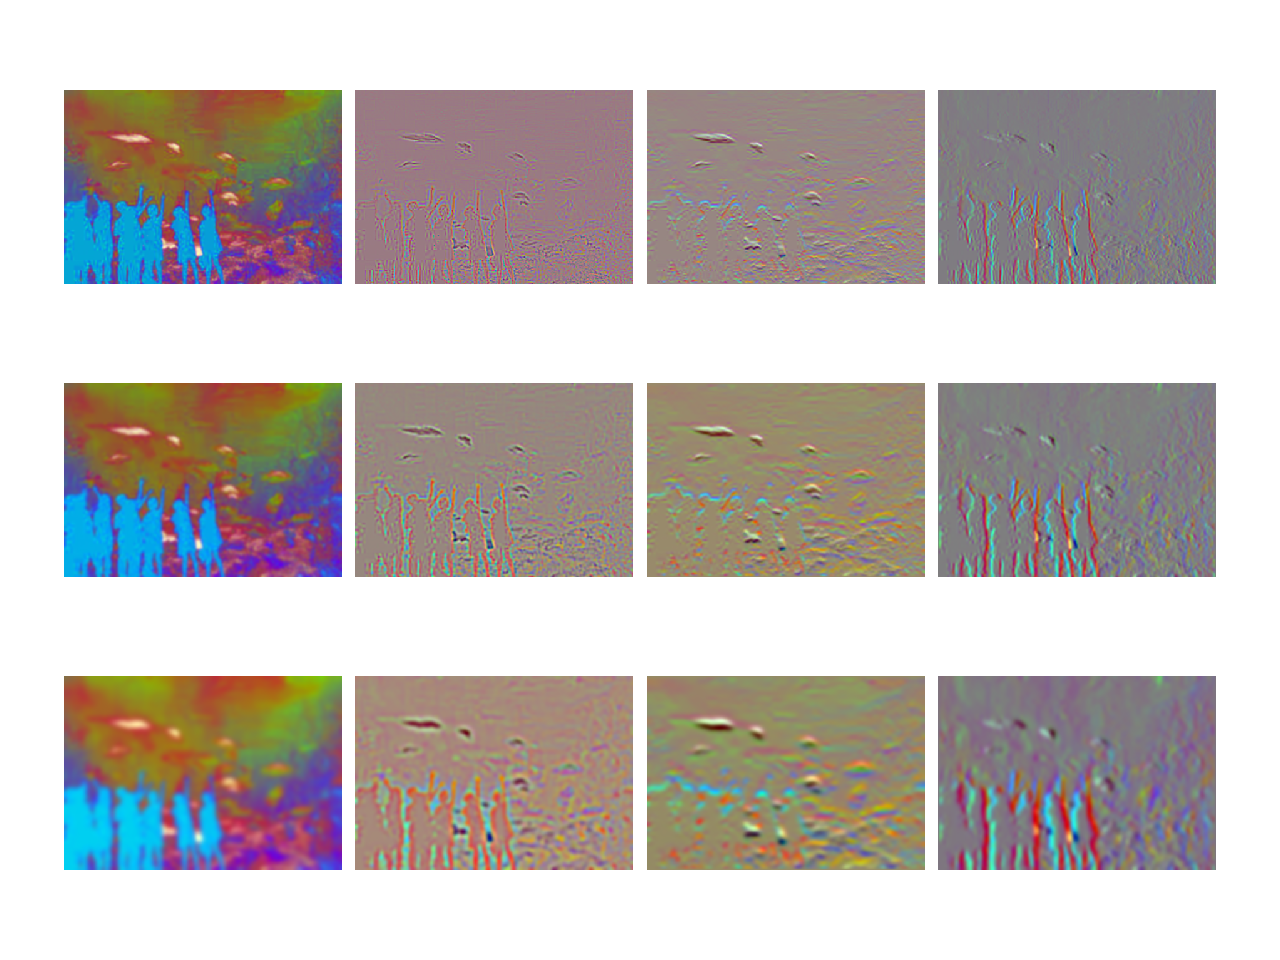
\includegraphics[width=0.6\textwidth]{results/1_1_2_aquarium.png}
\caption{collage of images}
\end{figure}

\newpage
\setcounter{subsection}{2}
\subsection{Computing Visual Words}

Image1: /kitchen/sun\_aasmevtpkslccptd.jpg

\begin{figure}[H]
\centering
\subfigure[RGB image]{
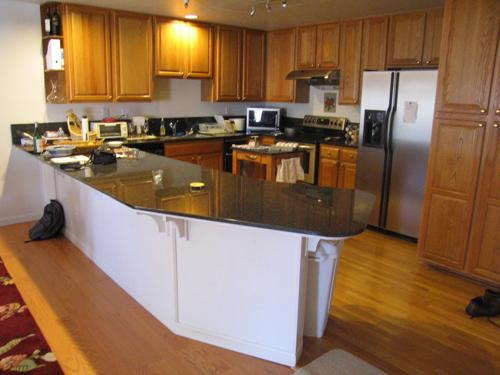
\includegraphics[width = 0.4\textwidth]{results/sun_aasmevtpkslccptd.jpg}}
\subfigure[wordmap]{
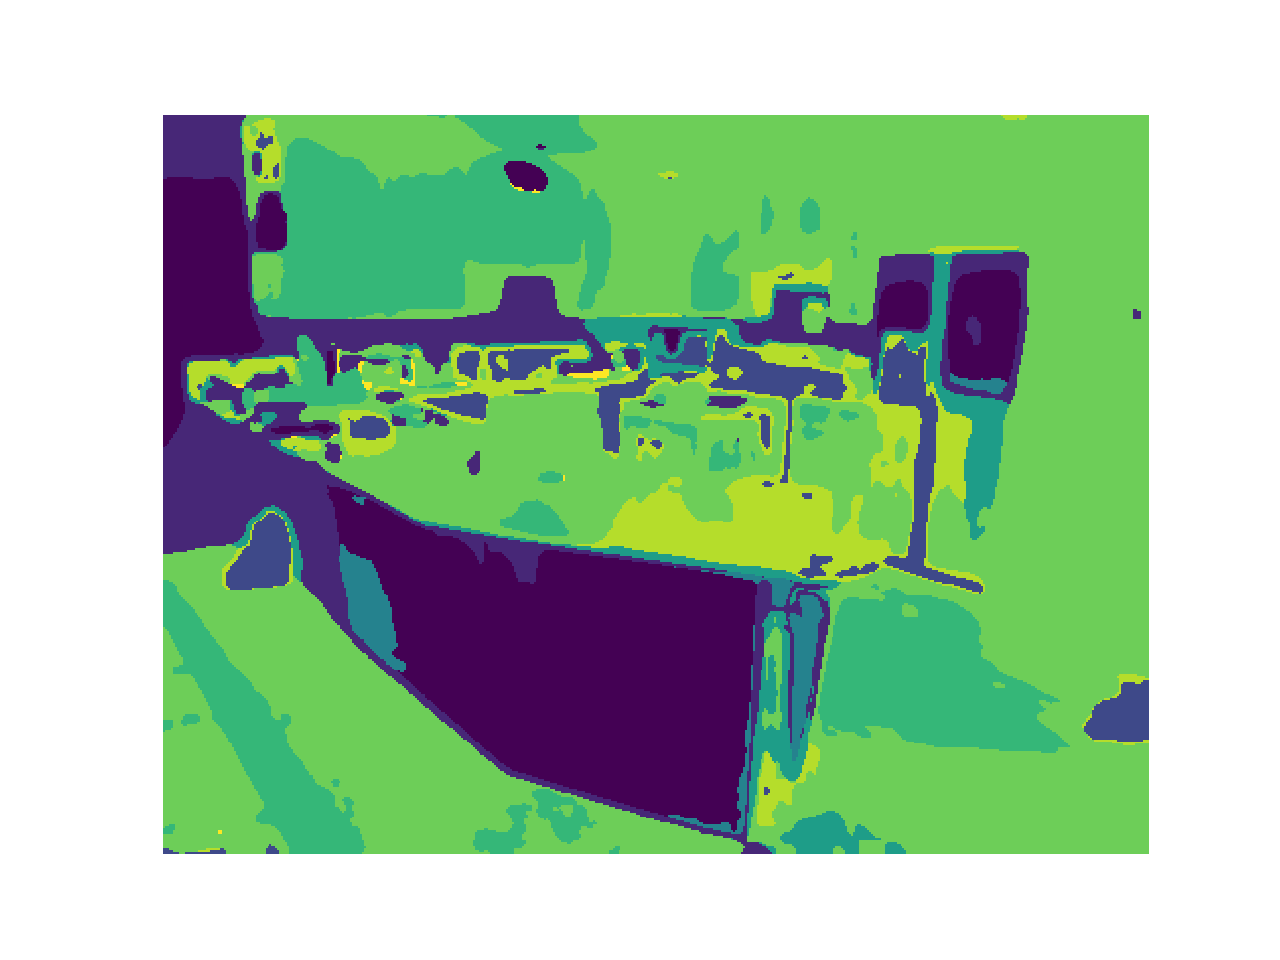
\includegraphics[width = 0.4\textwidth]{results/1_3_kitchen.png}}
\end{figure}

Image2: /highway/sun\_aqpxkrnzgghnpmvu.jpg

\begin{figure}[H]
\centering
\subfigure[RGB image]{
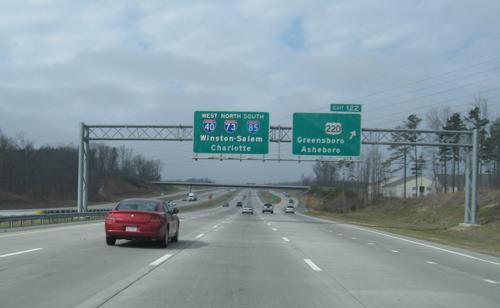
\includegraphics[width = 0.4\textwidth]{results/sun_aqpxkrnzgghnpmvu.jpg}}
\subfigure[wordmap]{
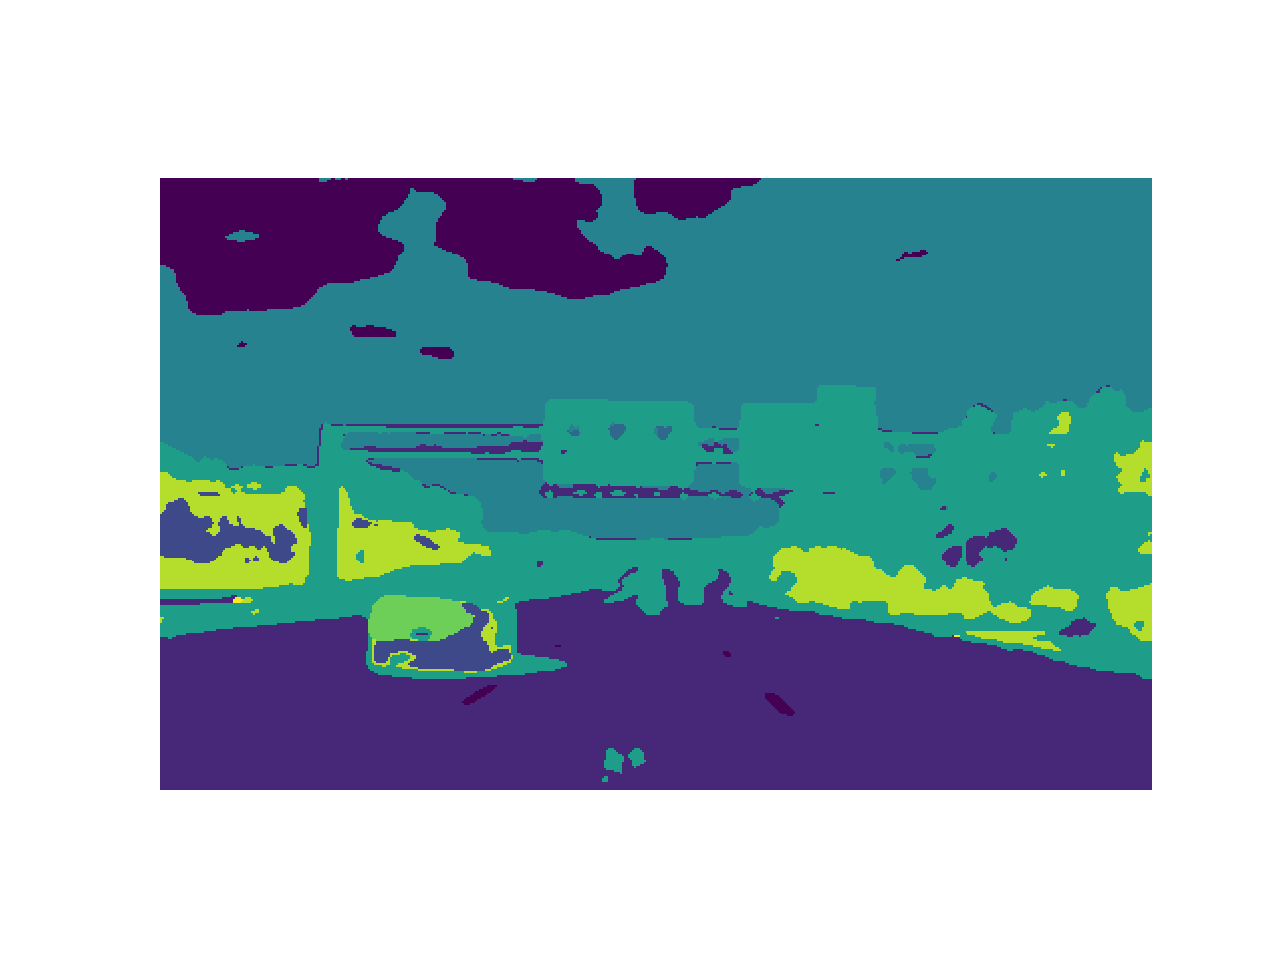
\includegraphics[width = 0.4\textwidth]{results/1_3_highway.png}}
\end{figure}

Image3: /waterfall/sun\_bjgujnjeakwxtjtz.jpg

\begin{figure}[H]
\centering
\subfigure[RGB image]{
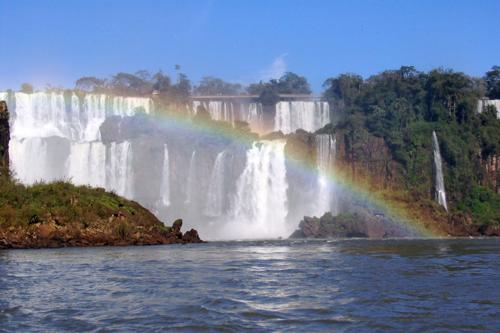
\includegraphics[width = 0.4\textwidth]{results/sun_bjgujnjeakwxtjtz.jpg}}
\subfigure[wordmap]{
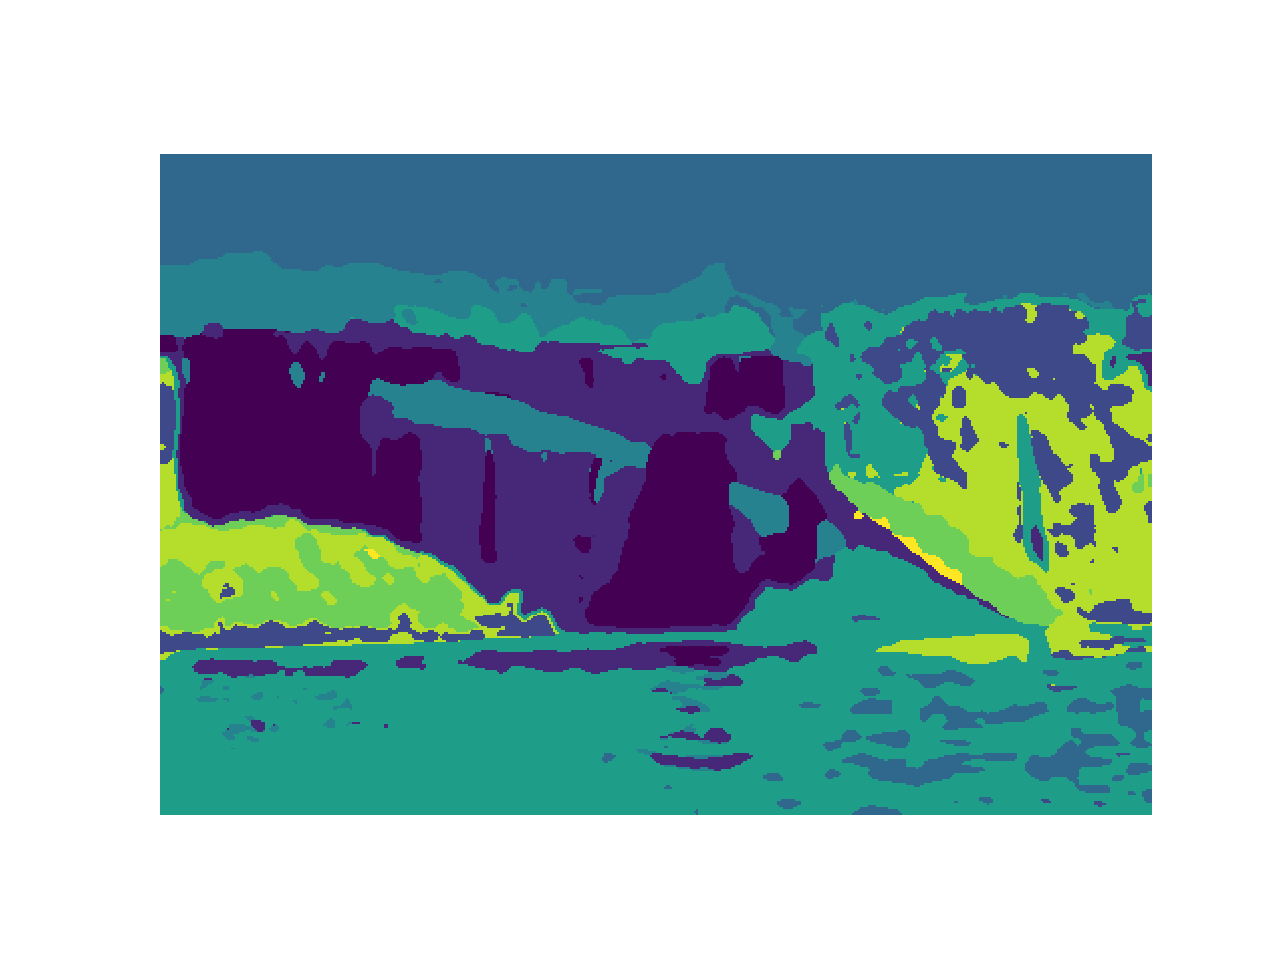
\includegraphics[width = 0.4\textwidth]{results/1_3_waterfall.png}}
\end{figure}
Comment: The "word" boundaries could be matched with the highlights, shadows, contours and blobs in RGB images easily.

\section{Building a Recognition System}
\setcounter{subsection}{4}
\subsection{Quantitative Evaluation}

With default parameters $K = 10$, $L = 2$, the confusion matrix is shown below:

\begin{figure}[H]
\centering
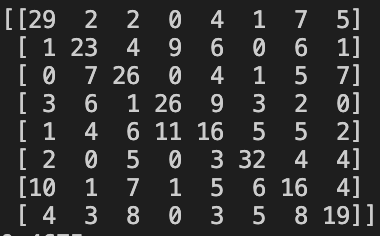
\includegraphics[width=0.6\textwidth]{results/default_mat.png}
\caption{confusion matrix}
\end{figure}

The accuracy is $46.75\%$

\setcounter{subsection}{5}
\subsection{Find the Failures}

Many aquarium images are classified as waterfall.

Sample: sun\_aqzlijeqktetgrtd.jpg

\begin{figure}[H]
\centering
\subfigure[RGB image]{
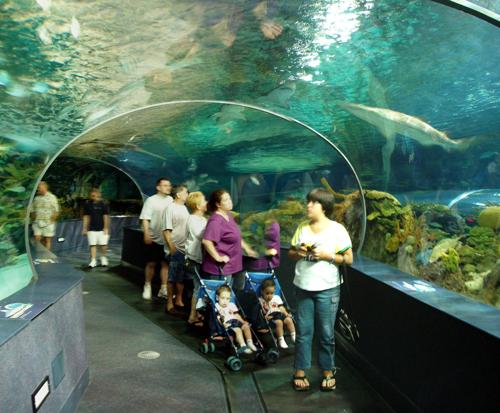
\includegraphics[width = 0.3\textwidth]{data/aquarium/sun_aqzlijeqktetgrtd.jpg}}
\subfigure[wordmap]{
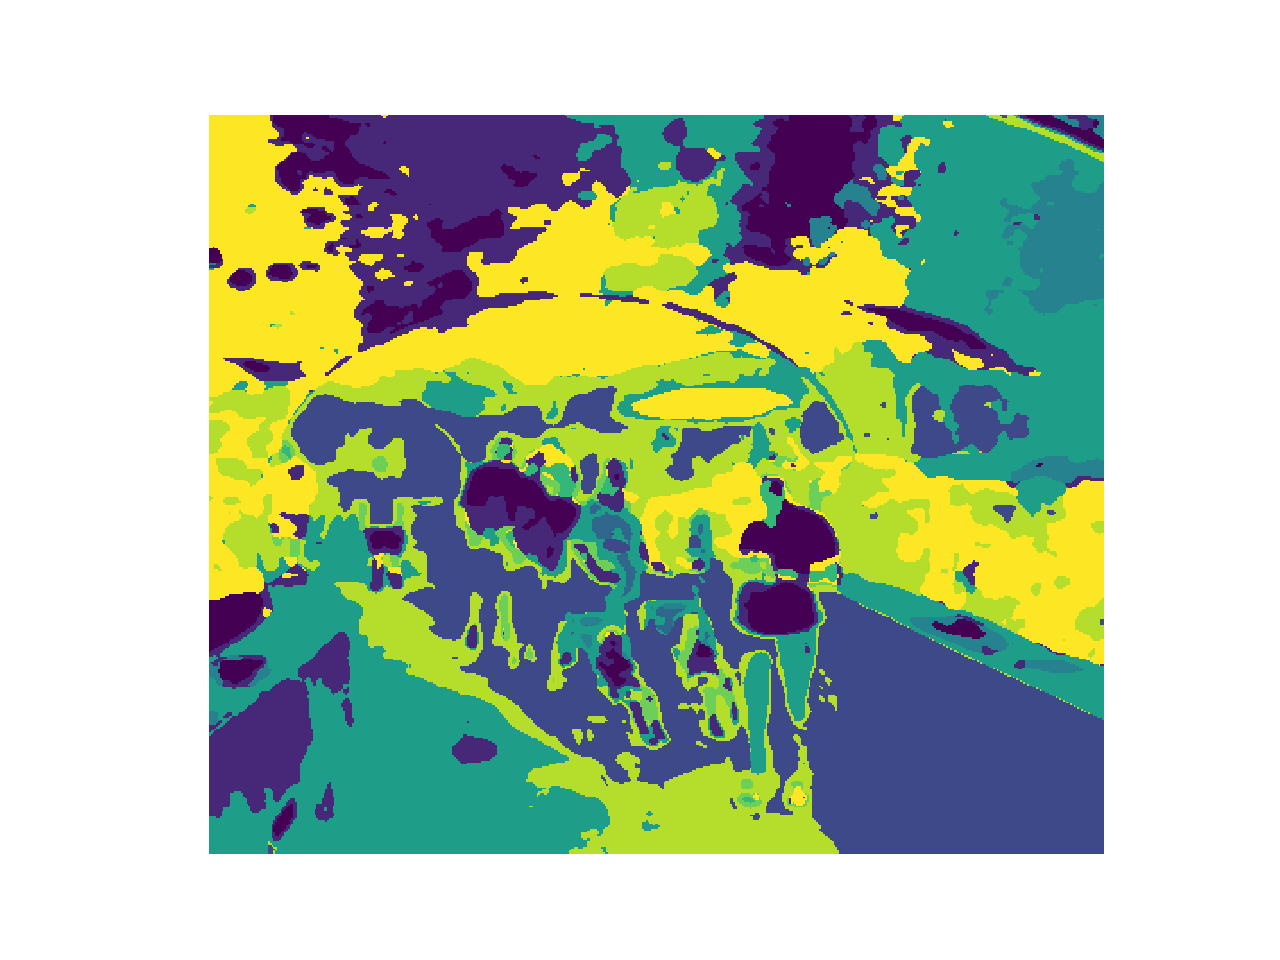
\includegraphics[width = 0.4\textwidth]{results/Figure_2.png}}
\end{figure}

The wordmap contains large amount of green and yellow which resembles the nature sight of waterfall.

\section{Improving Performance}
\setcounter{subsection}{0}
\subsection{Hyperparameter Tuning}

At first step I tuned $K$ from $10$ to $30$ and tuned $L$ from $2$ to $3$, and using scales $\left[ \begin{smallmatrix} 1 & 2 & 4 \end{smallmatrix} \right]$ the accuracy increased from $46.75\%$ to $56\%$.

At second step I changed $L$ to $4$ and changed $alpha$ from $25$ to $50$, then I achieved accuracy $59.25\%$.

With $alpha$ increased to $75$ and all other parameters remain the same, the accuracy dropped to $58.5\%$.

With $alpha = 50$, $K = 100$, $L = 4$, scales = $\left[ \begin{smallmatrix} 1 & 2 & 4 & 8 \end{smallmatrix} \right]$, I achieved accuracy $60\%$.

\end{document}
